\documentclass{ctexart}
\usepackage{amsmath,amssymb,amsthm,bm}
\usepackage{xcolor}
\definecolor{Solarized-base03}{RGB}{0, 43, 54}
\definecolor{Solarized-base02}{RGB}{7, 54, 66}
\definecolor{Solarized-base01}{RGB}{88, 110, 117}
\definecolor{Solarized-base00}{RGB}{101, 123, 131}
\definecolor{Solarized-base0}{RGB}{131, 148, 150}
\definecolor{Solarized-base1}{RGB}{147, 161, 161}
\definecolor{Solarized-base2}{RGB}{238, 232, 213}
\definecolor{Solarized-base3}{RGB}{253, 246, 227}
\definecolor{Solarized-yellow}{RGB}{181, 137, 0}
\definecolor{Solarized-orange}{RGB}{203, 75, 22}
\definecolor{Solarized-red}{RGB}{220, 50, 47}
\definecolor{Solarized-magenta}{RGB}{211, 54, 130}
\definecolor{Solarized-violet}{RGB}{108, 113, 196}
\definecolor{Solarized-blue}{RGB}{38, 139, 210}
\definecolor{Solarized-cyan}{RGB}{42, 161, 152}
\definecolor{Solarized-green}{RGB}{133, 153, 0}
\color{Solarized-base01}
\pagecolor{Solarized-base3}

\newcommand{\red}[1]{\textcolor{Solarized-red}{#1}}
\newcommand{\yellow}[1]{\textcolor{Solarized-yellow}{#1}}
\newcommand{\blue}[1]{\textcolor{Solarized-blue}{#1}}
\newcommand{\cyan}[1]{\textcolor{Solarized-cyan}{#1}}
\newcommand{\violet}[1]{\textcolor{Solarized-violet}{#1}}

\usepackage{fullpage}
\usepackage{graphicx,epsfig,subfigure}
\usepackage{tikz,pgfplots}
\pgfplotsset{compat=1.17}
\usepackage{ifthen}
\usetikzlibrary{backgrounds,automata,shapes,snakes,arrows,arrows.meta,chains,positioning,calc}

%%%%%% 下面两行字体设置需根据自己的系统调整
\setmainfont[]{EBGaramond08-Regular}
\setCJKmainfont[BoldFont=FZHei-B01]{FZLongZhao-R-GB}
%%%%%%
\xeCJKsetup{CJKmath=true}
\everymath{\color{Solarized-magenta}}

\def \zerov {\bm{0}}
\def \av {\bm{a}}
\def \bv {\bm{b}}
\def \cv {\bm{c}}
\def \dv {\bm{d}}
\def \ev {\bm{e}}
\def \fv {\bm{f}}
\def \gv {\bm{g}}
\def \hv {\bm{h}}
\def \pv {\bm{p}}
\def \tv {\bm{t}}
\def \uv {\bm{u}}
\def \vv {\bm{v}}
\def \wv {\bm{w}}
\def \xv {\bm{x}}
\def \yv {\bm{y}}
\def \zv {\bm{z}}

\def \Av {\mathbf{A}}
\def \Bv {\mathbf{B}}
\def \Cv {\mathbf{C}}
\def \Dv {\mathbf{D}}
\def \Fv {\mathbf{F}}
\def \Gv {\mathbf{G}}
\def \Hv {\mathbf{H}}
\def \Iv {\mathbf{I}}
\def \Kv {\mathbf{K}}
\def \Lv {\mathbf{L}}
\def \Mv {\mathbf{M}}
\def \Pv {\mathbf{P}}
\def \Qv {\mathbf{Q}}
\def \Sv {\mathbf{S}}
\def \Uv {\mathbf{U}}
\def \Vv {\mathbf{V}}
\def \Wv {\mathbf{W}}
\def \Xv {\mathbf{X}}
\def \Yv {\mathbf{Y}}
\def \Zv {\mathbf{Z}}

\def \alphav {\bm{\alpha}}
\def \betav {\bm{\beta}}
\def \gammav {\bm{\gamma}}
\def \lambdav {\bm{\lambda}}
\def \Lambdav {\bm{\Lambda}}
\def \thetav {\bm{\theta}}
\def \epsilonv {\bm{\epsilon}}
\def \xiv {\bm{\xi}}
\def \muv {\bm{\mu}}
\def \Sigmav {\bm{\Sigma}}
\def \Phiv {\bm{\Phi}}
\def \nuv {\bm{\nu}}

\def \Acal {\mathcal{A}}
\def \Bcal {\mathcal{B}}
\def \Ical {\mathcal{I}}
\def \Lcal {\mathcal{L}}
\def \Ncal {\mathcal{N}}
\def \Pcal {\mathcal{P}}

\def \Dbb {\mathbb{D}}
\def \Ebb {\mathbb{E}}
\def \Nbb {\mathbb{N}}
\def \Qbb {\mathbb{Q}}
\def \Rbb {\mathbb{R}}
\def \Sbb {\mathbb{S}}

\def \Ifrak {\mathfrak{I}}
\def \Lfrak {\mathfrak{L}}
\def \Pfrak {\mathfrak{P}}

\def \diag {\mathrm{diag}}
\def \sign {\mathrm{sign}}
\def \sp {\mathrm{span}}
\def \diff {\mathrm{d}}
\def \tr {\mathrm{tr}}
\def \KL {\mathrm{KL}}
\def \var {\mathrm{var}}
\def \cov {\mathrm{cov}}
\def \ow {\mathrm{o.w.}}

\def \st {\mbox{s.t.}}
\def \const {\mbox{const}}

\DeclareMathOperator*{\argmin}{argmin}
\DeclareMathOperator*{\argmax}{argmax}

\allowdisplaybreaks[4]

\begin{document}
\title{}
\author{}
\date{}
\maketitle

\begin{figure}[ht]
    \centering
    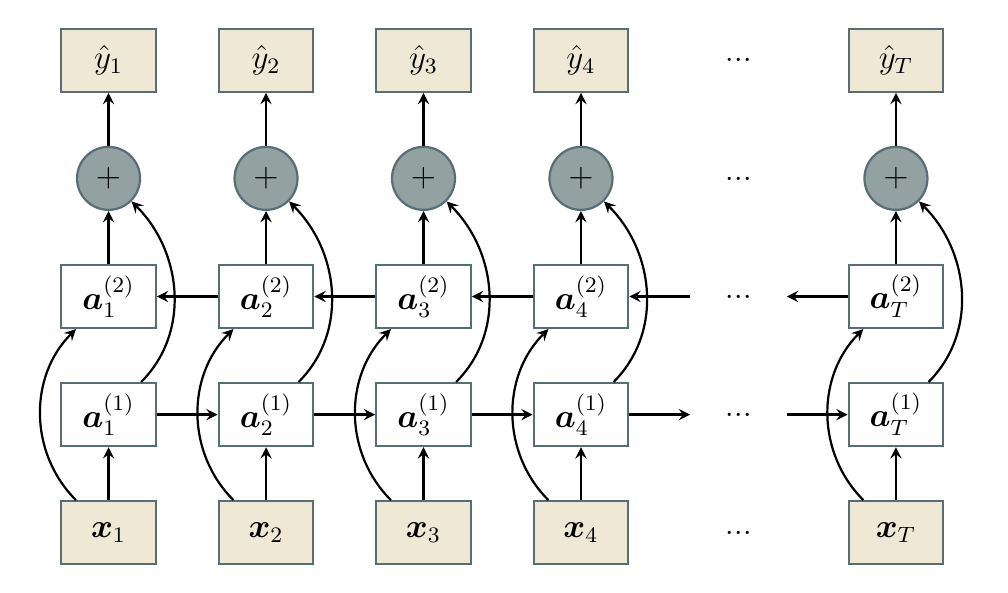
\begin{tikzpicture} [
            thick, >=stealth, scale=1, font=\large,
            minimum-size/.style = {minimum height=0.8cm, minimum width=1.2cm},
            plain/.style = {draw=none, minimum-size}, % 倒数第二列
            hidden/.style = {rectangle, minimum-size, draw=Solarized-base01}, % 隐藏层
            io/.style = {hidden, fill=Solarized-base2}, % 输入输出层
            add/.style = {circle, minimum height=0.8cm, draw=Solarized-base01, fill=Solarized-base1} % 加号
        ]

        \pgfmathsetmacro{\xinc}{2};
        \pgfmathsetmacro{\yinc}{1.5};

        \def \indexs {{1, 2, 3, 4, 5, "T"}};
        \def \names {{"\xv", "\av^{(1)}", "\av^{(2)}", "+", "\hat{y}"}};
        \def \styles {{"io", "hidden", "hidden", "add", "io"}};

        \foreach \i in {0, ..., 5}{

                \ifthenelse{\NOT \i = 4}{ % 非倒数第二列

                    \pgfmathparse{\indexs[\i]};
                    \edef \index {\pgfmathresult}; % 获取下标

                    \foreach \j [count=\jj from -1] in {0, ..., 4}{

                            \pgfmathparse{\styles[\j]};
                            \edef \style {\pgfmathresult}; % 获取样式

                            \ifthenelse{\j = 3}{ % 加号那一行不需要下标
                                \node [{\style}] (\i\j) at (\i*\xinc, \j*\yinc) {$\pgfmathparse{\names[\j]}\pgfmathresult$};
                            }{
                                \node [{\style}] (\i\j) at (\i*\xinc, \j*\yinc) {$\pgfmathparse{\names[\j]}\pgfmathresult_\index$};
                            }

                            \ifthenelse{\NOT \j = 0 \AND \NOT \j = 2}{
                                \draw[->] (\i\jj) -- (\i\j);
                            }{;}

                            \ifthenelse{\j = 2}{ % 画跳连边
                                \draw[->] (\i0) to [out=135, in=225] (\i2);
                            }{;}

                            \ifthenelse{\j = 3}{ % 画跳连边
                                \draw[->] (\i1) to [out=45, in=315] (\i3);
                            }{;}
                        }
                }{
                    \foreach \j in {0, ..., 4}{
                            \node [plain] (\i\j) at (\i*\xinc, \j*\yinc) {...};
                        }
                }
            }

        \foreach \i [count=\ii] in {0, ..., 5}{ % 画横向边
                \ifthenelse{\i < 5}{
                    \draw[->] (\i1) -- (\ii1);
                    \draw[->] (\ii2) -- (\i2);
                }{;}
            }

    \end{tikzpicture}
    \caption{双向循环神经网络}
\end{figure}




\end{document}

